\documentclass{article}
\usepackage{graphicx}
\graphicspath{ {Home/Desktop/DScourseS24/ProblemSets/ProblemSet6} }

\title{PS6 Felkner}
\author{Beth Felkner}
\date{March 2024}

\begin{document}

\maketitle

\section{Data Cleaning and Transformation}
My dataset is career stats by year for Adrian Beltre, an MLB third baseman who was recently inducted into the 2024 Hall oF Fame class with a near unanimous vote. The dataset did not need very much cleaning, because it was already a nicely compiled and published dataset as opposed to "wild" data. The only cleaning I really did is remove some extraneous rows about Beltre's minor league stats that I did not want. I did some transformation specific to the visualizations that I wanted to make. For my first visualization, I wanted to include All-Star status as a factor variable on top of a continuous numeric variable (batting average), so I just created a dummy variable with "Yes" or "No" for each year. For my second visualization which is about tenure with his teams, I wanted to clearly reflect the team name and tenure in my legend, so I transformed the Tm variable from just an abbreviation to the full team team with the tenure in parentheses. My third visualization did not require any specific transformation.

\section{Visualization 1: Beltre Batting Average with All-Stars Years Highlighted}
    \centering
    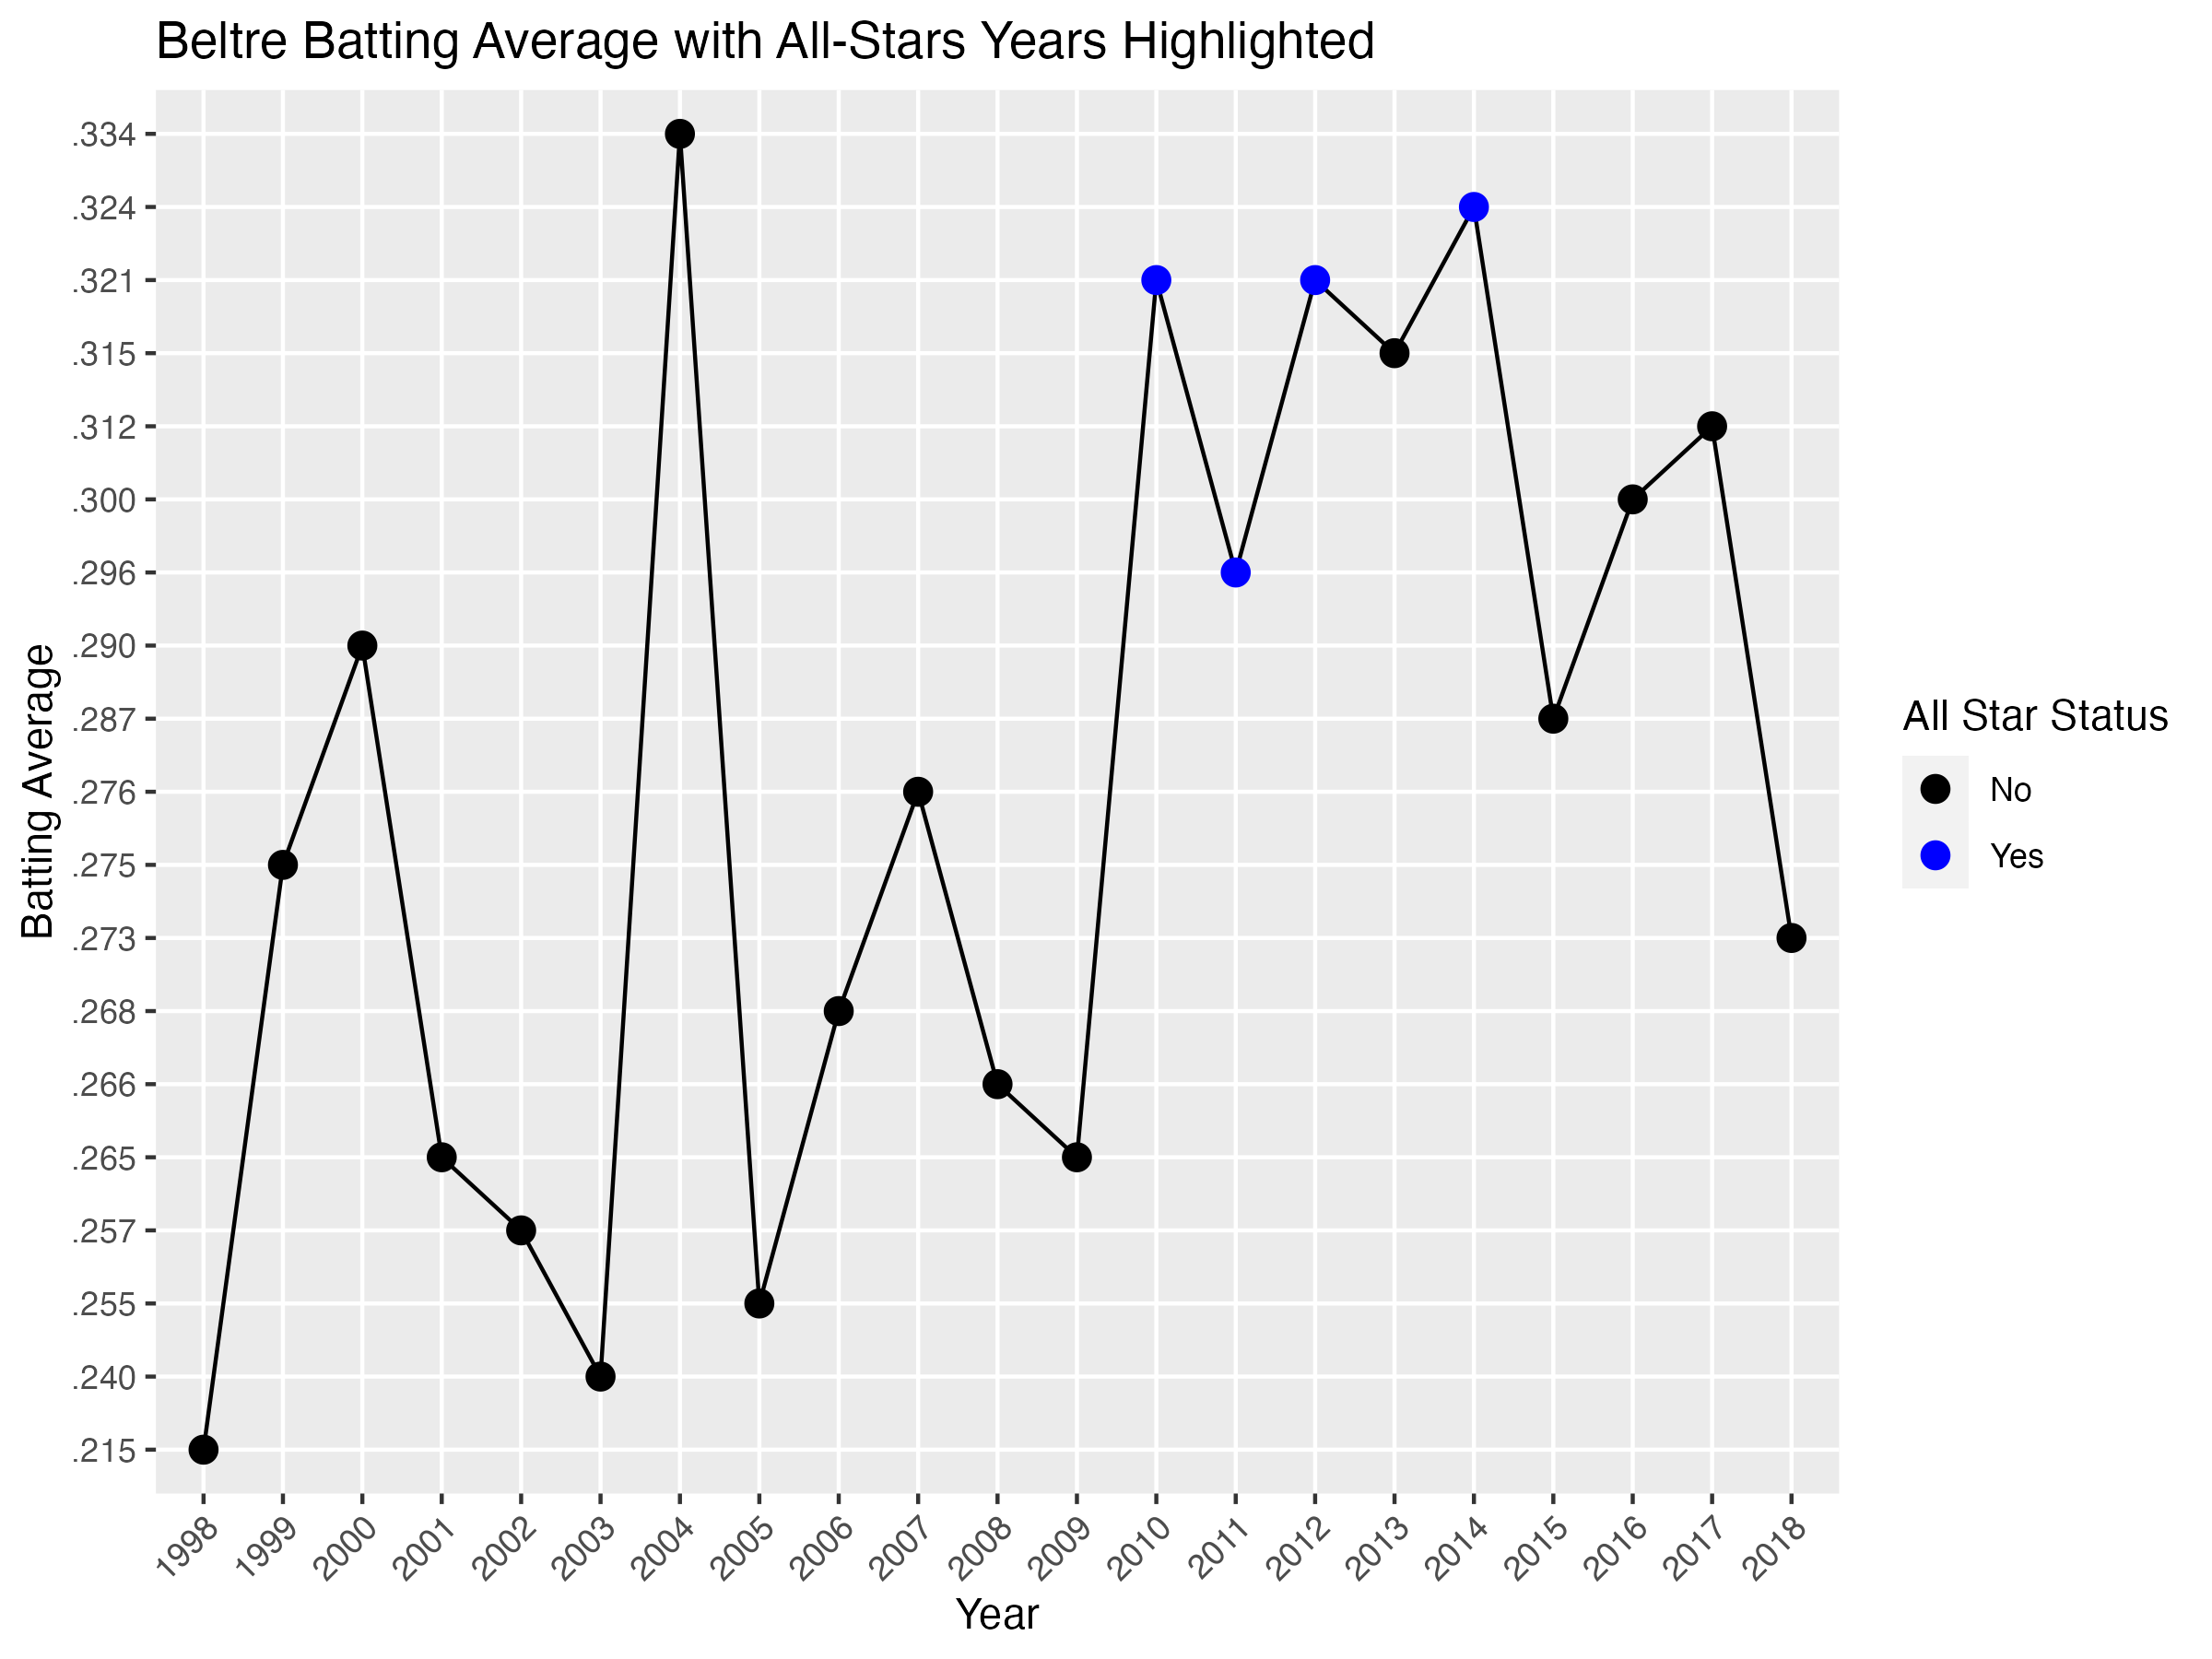
\includegraphics[width=15cm]{PS6a_Felkner.png}
This visualization simultaneously shows Beltre's yearly batting average along with his status as an All-Star or not. They are helpful to me understanding the data set because it allows us to see what factors may affect All-Star status (which is fan voted). In general he is an All Star when he has a higher average, but in 2004 he had an extremely high average and was not, which suggests that length of career/established reputation is also a factor in addition to just pure stats. 

\section{Visualization 2: Beltre Career by Tenure with Each Team}
    \centering
    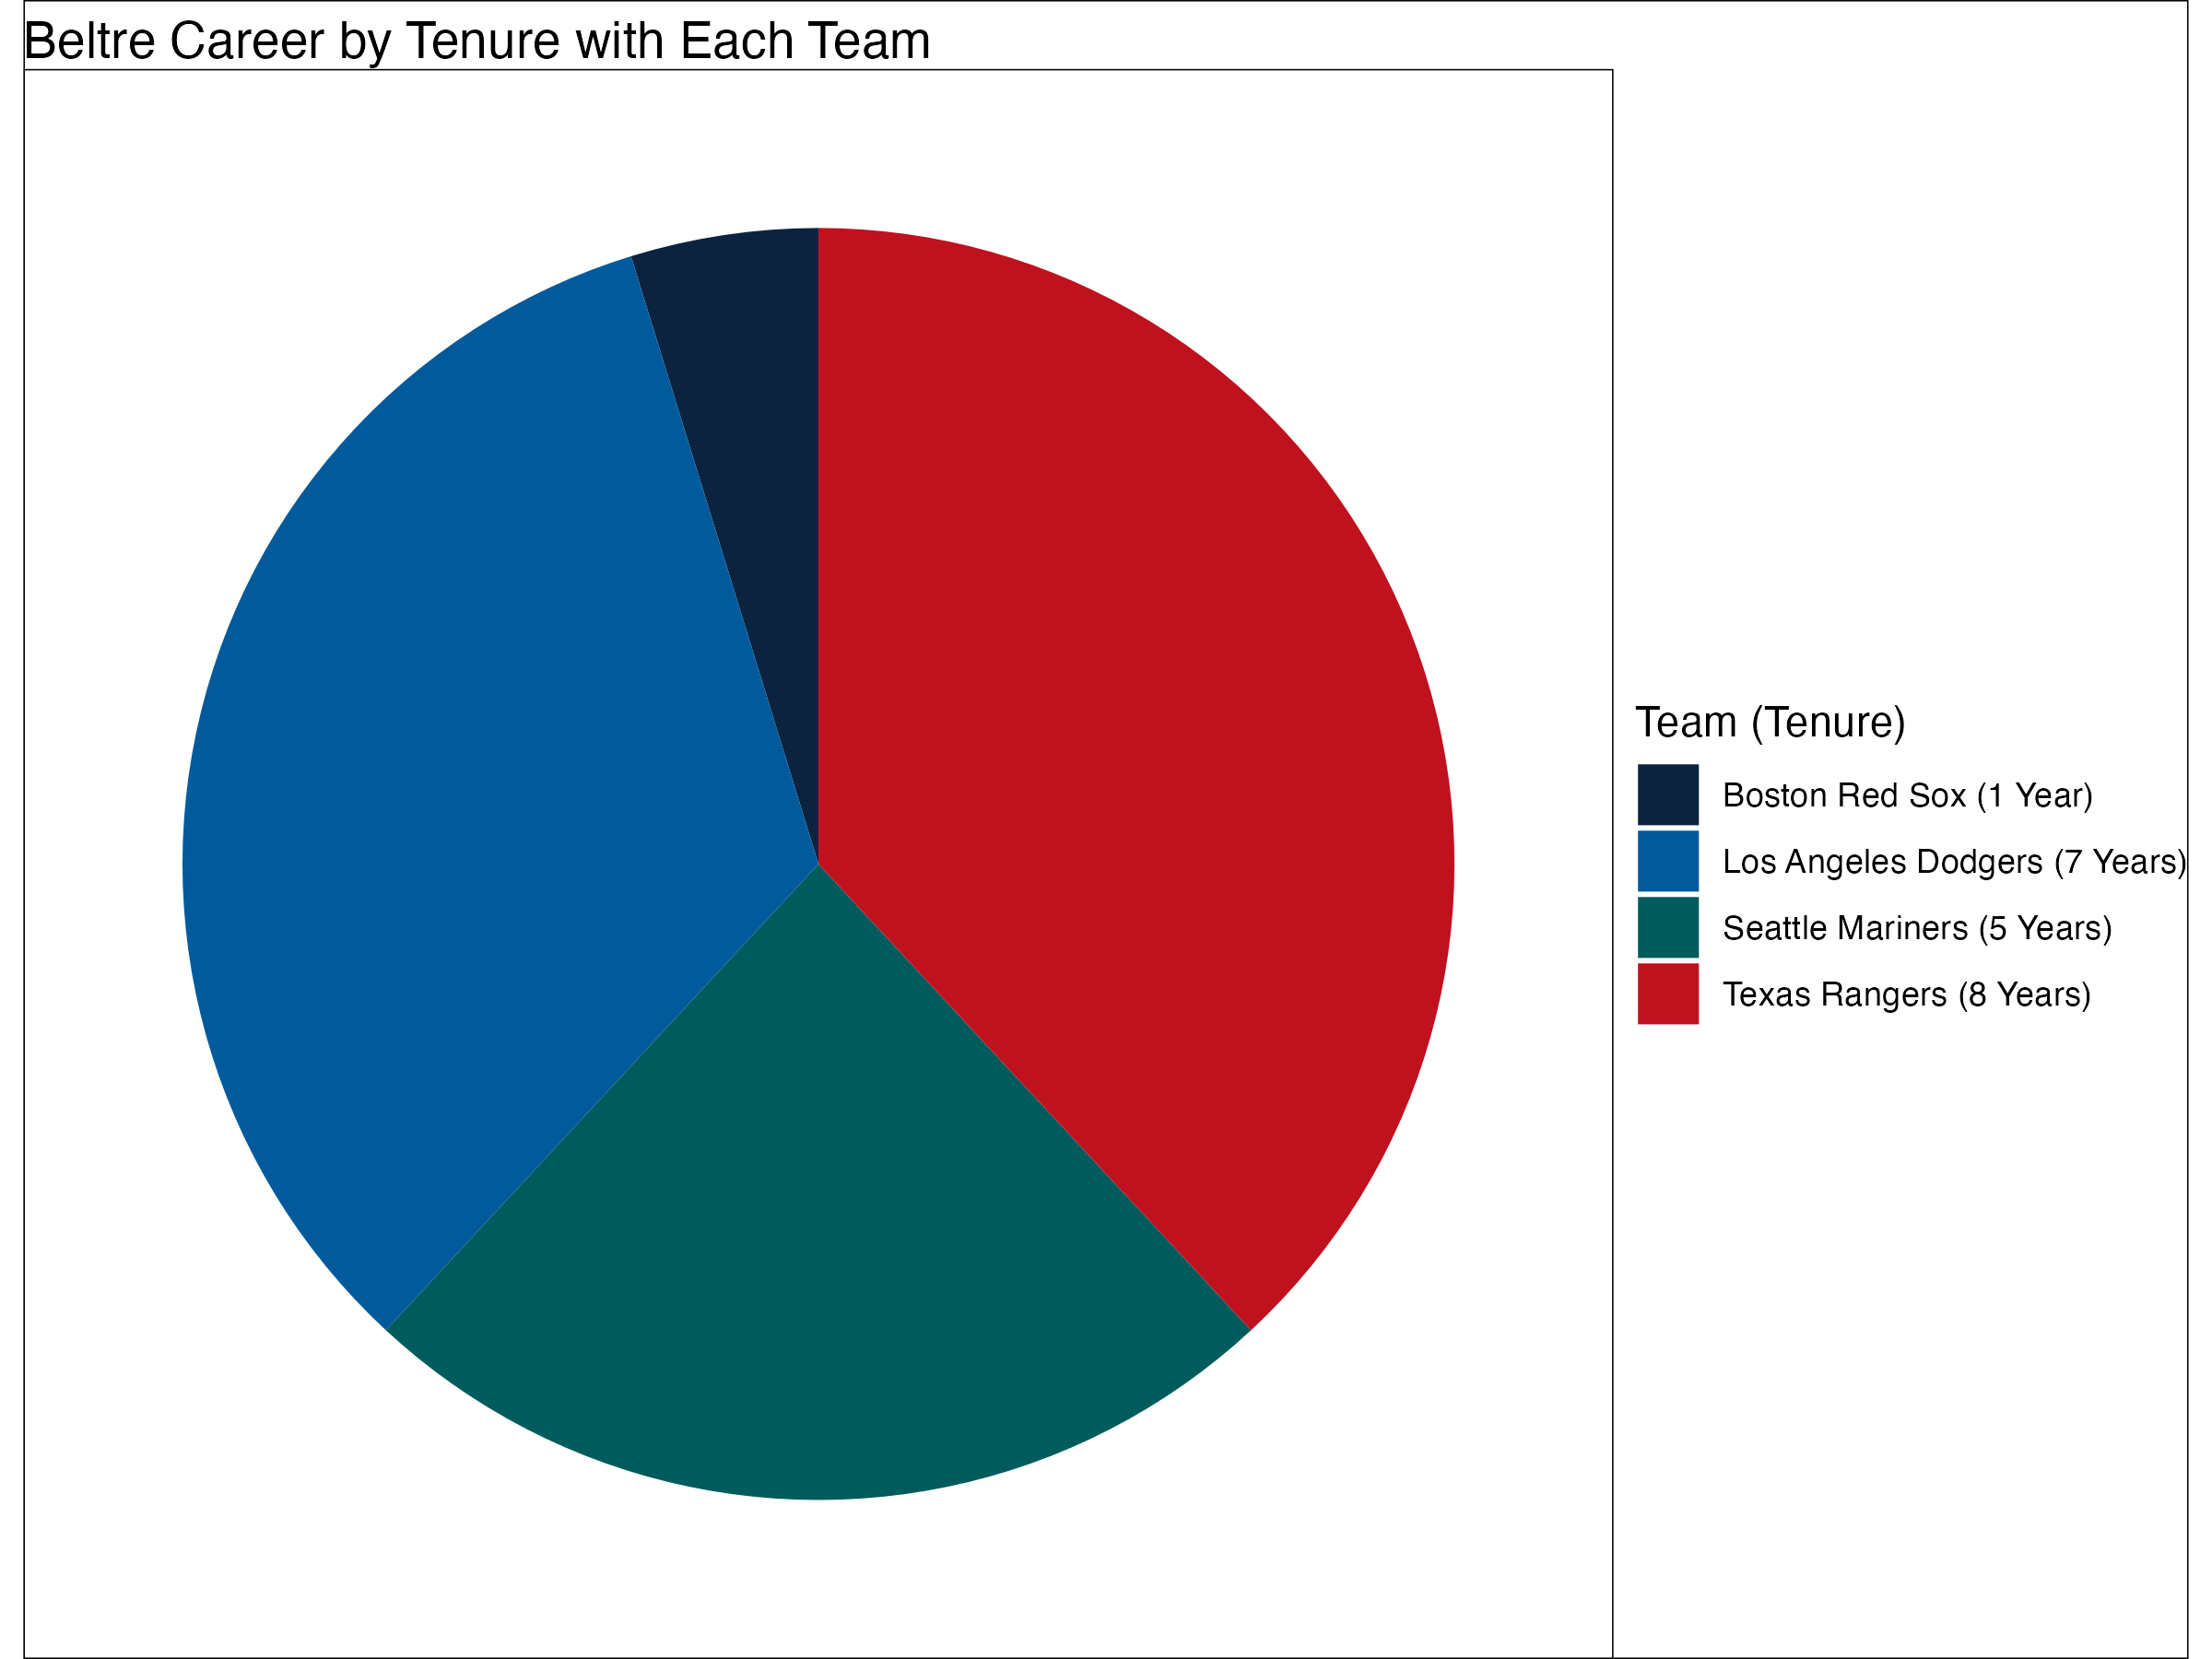
\includegraphics[width=15cm]{PS6b_Felkner.png}
This visualization shows the tenure Beltre spent with each of the four teams he played for as a proportion of his total career. I wanted to make a visualization that incorpated the actual team colors (I used their official team hex codes in my script), and I thought about trying to add team color as a layer on top of some other stat but I thought that might get convoluted, so I just kept it simple on this one. I do think its useful in terms of conceptualizing his full career though, because I tend to think of him only as a Ranger but he actually spent a significant amount of time with other teams as well. 

\section{Visualization 3: Beltre Walks vs On Base Percentage}
    \centering
    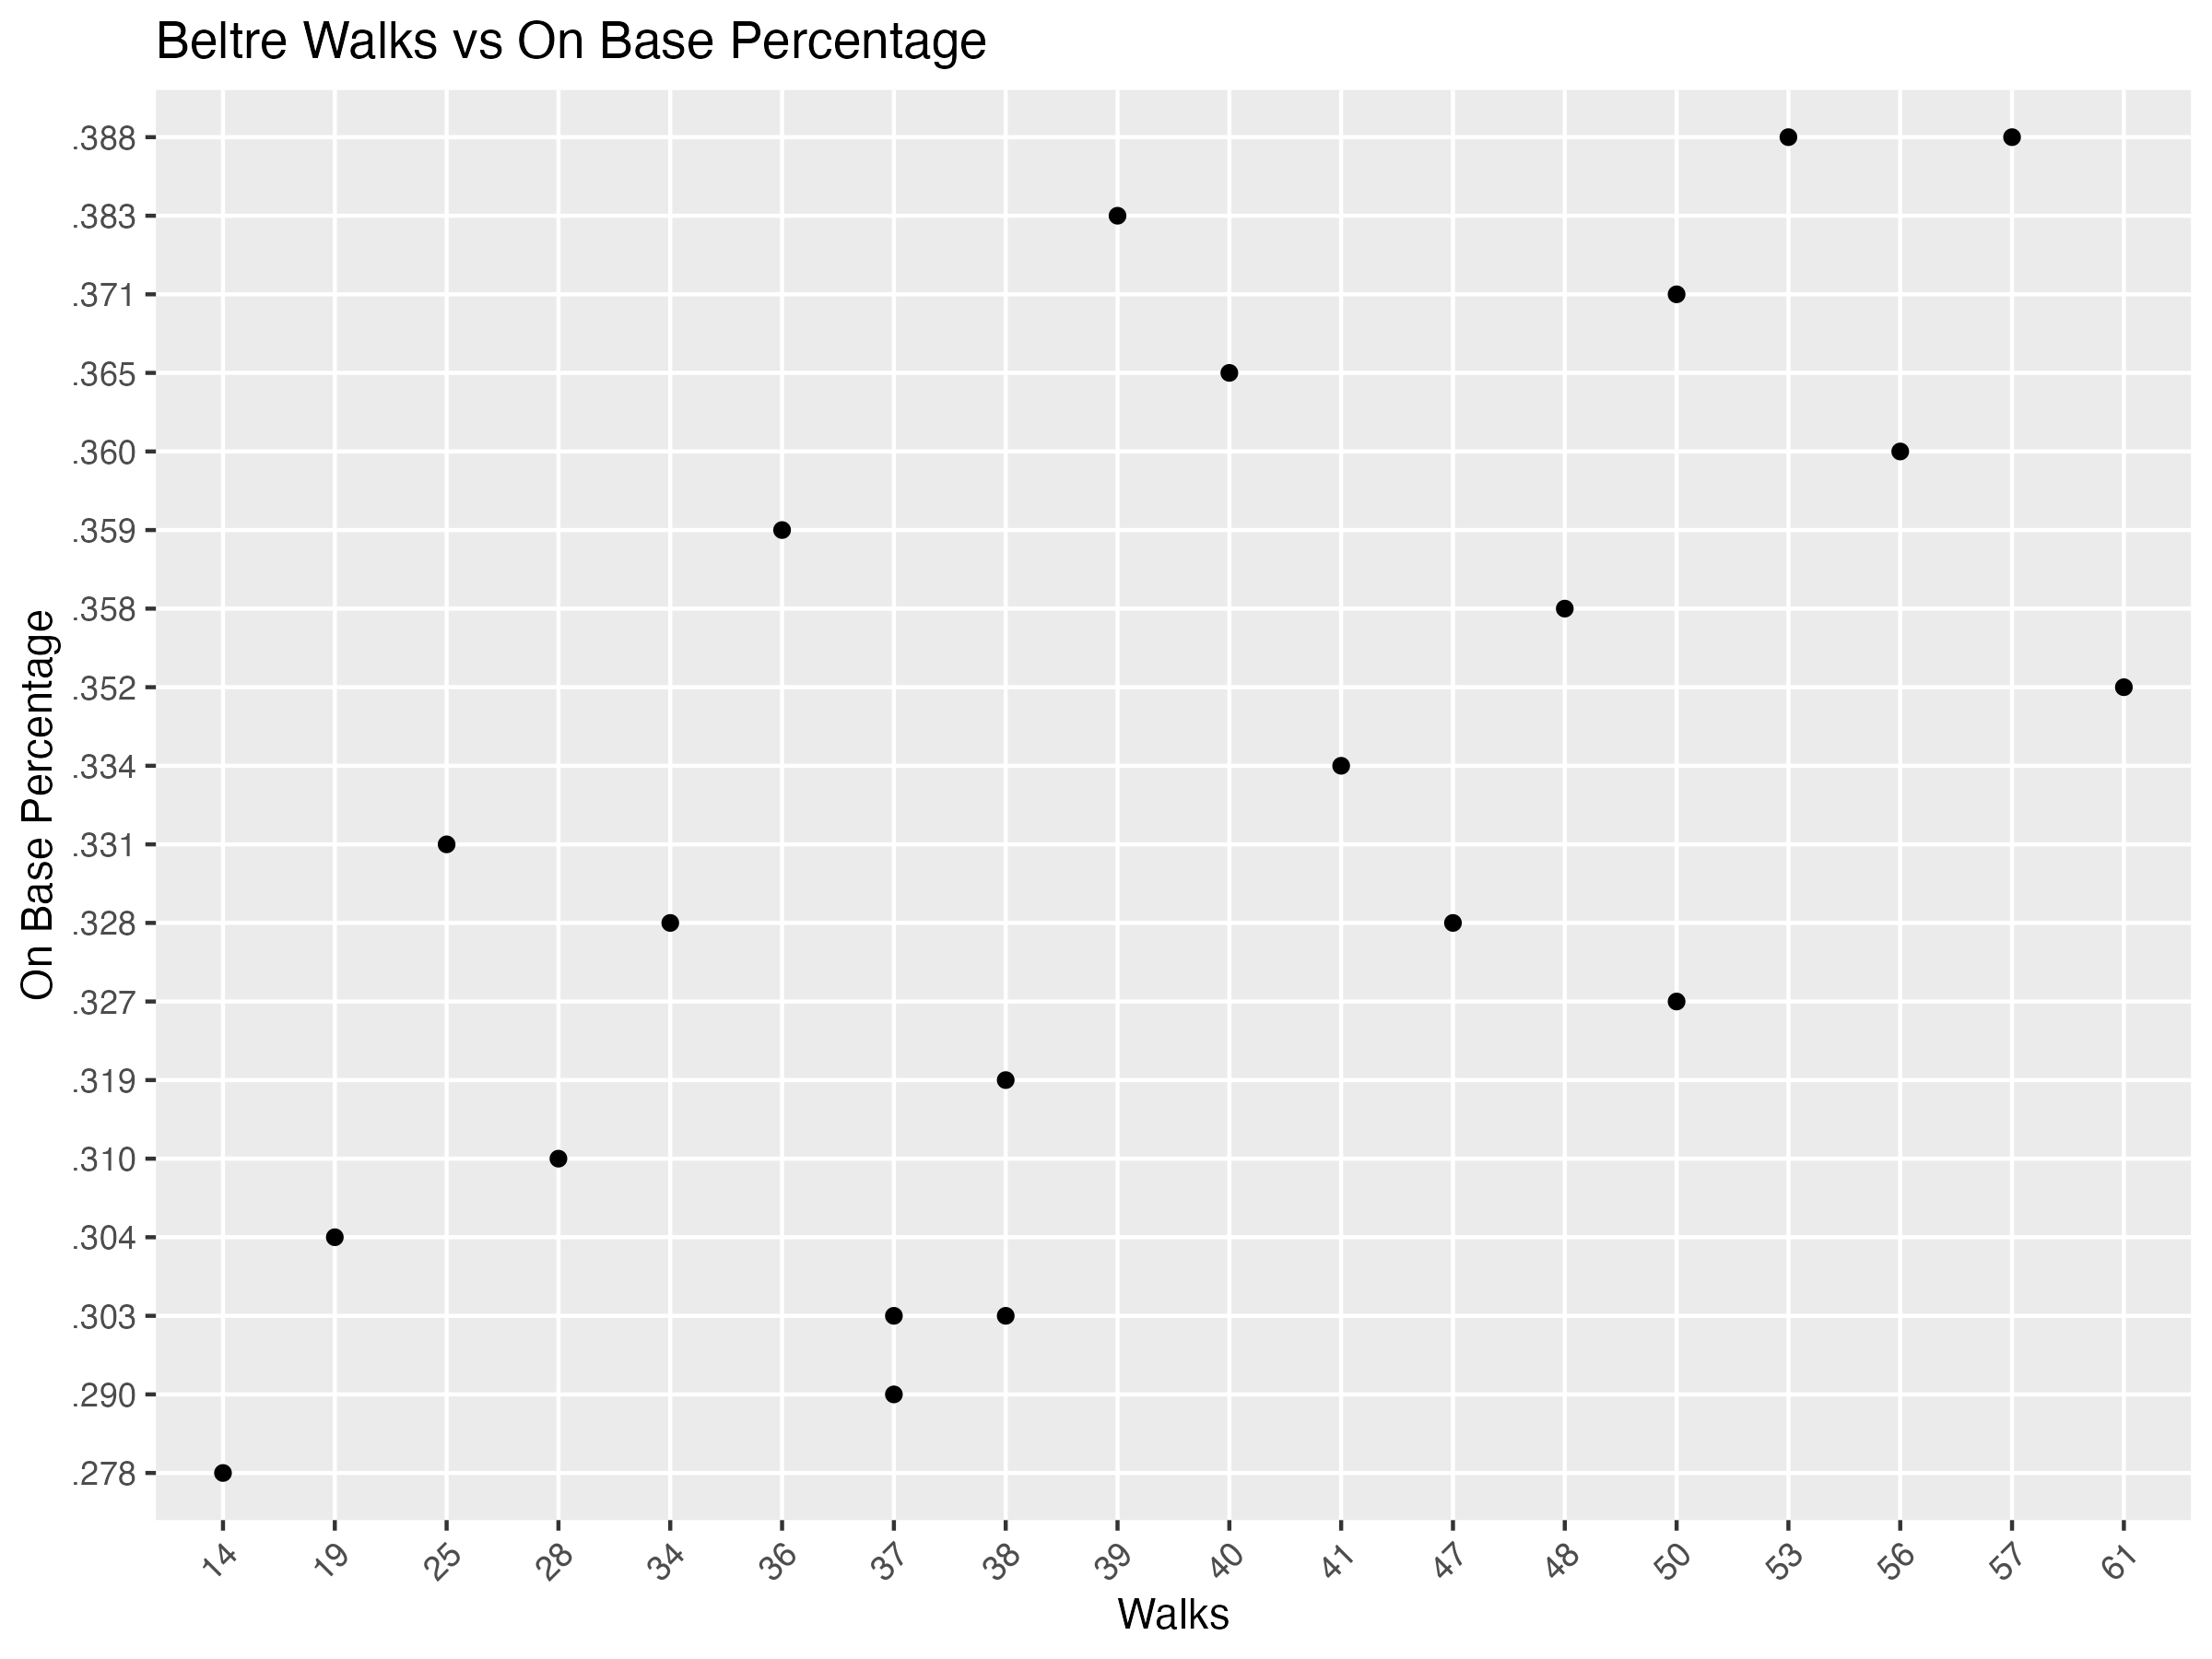
\includegraphics[width=15cm]{PS6c_Felkner.png}
This scatterplot shows the relationship between walks and on base percentage in a given season. We can see that there is a clear positive, roughly linear trend between the two. I wanted to visualize that relationship for Beltre, because common sense would hold  that more walks will obviously lead to a higher OBP, but it's possible that could change if a player becomes less aggressive at the plate trying to draw walks but then also starts striking out looking a lot. But for Beltre at least, we can see thats not the case.

\end{document}
